\documentclass[11pt,a4paper]{article}

% ---------- house style (as teacher_attrition_brief.tex) ----------
\usepackage[T1]{fontenc}
\usepackage[utf8]{inputenc}
\usepackage{tgtermes}
\usepackage[margin=2.5cm,top=2.4cm,bottom=2.6cm]{geometry}
\usepackage{graphicx,booktabs,xcolor,colortbl,tcolorbox,caption,enumitem,setspace,amsmath,float}
\usepackage[hidelinks]{hyperref}

\definecolor{ecnavy}{HTML}{12355B}
\definecolor{ecyellow}{HTML}{FFCD00}
\definecolor{eccoral}{HTML}{E34948}
\definecolor{ecblue}{HTML}{2A78D6}
\definecolor{ecink}{HTML}{1A2430}
\definecolor{ecgray}{HTML}{5A6572}
\definecolor{ecpale}{HTML}{FFF8DC}

\captionsetup{font={small},labelfont={bf},
              justification=justified,singlelinecheck=false}
\makeatletter\setlength{\@fptop}{0pt}\makeatother
\renewcommand{\topfraction}{0.85}
\renewcommand{\bottomfraction}{0.6}
\renewcommand{\textfraction}{0.15}
\renewcommand{\floatpagefraction}{0.8}
\setlength{\parskip}{5pt}\setlength{\parindent}{0pt}
\linespread{1.14}
\color{ecink}

\newcommand{\fignote}[1]{\par\vspace{4pt}%
  \begin{minipage}{\linewidth}\footnotesize\color{ecgray}#1\end{minipage}}

\begin{document}

% ---------- title ----------
\vspace*{22pt}
\begin{center}
{\fontsize{20}{26}\selectfont\bfseries
A Borrowed Recovery?\par}
\vspace{8pt}
{\fontsize{15}{20}\selectfont\bfseries
The 2025 Teacher-Workforce Data for the United States\par}

\vspace{22pt}
{\large \href{https://sites.google.com/view/joseeliasduranroa}{José Elías
Durán Roa}\footnote{PhD Candidate in Economics, University of Alicante, and
Research Intern at the OECD Directorate for Education and Skills. E-mail\,
\href{mailto:joseelias.duranroa@ocde.org}{joseelias.duranroa@ocde.org} and
\href{mailto:joduran@ua.es}{joduran@ua.es}. The views expressed here are
mine and do not represent those of the OECD. All remaining errors are my
own.}}

\vspace{6pt}
{\small July 2026}
\end{center}

\vspace{10pt}
\begin{tcolorbox}[colback=ecpale,colframe=ecnavy,boxrule=0.9pt,
                  left=10pt,right=10pt,top=8pt,bottom=8pt]
{\bfseries In brief.} Five turbulent years after the pandemic first hit
American classrooms, the 2025 workforce data read almost calm. Almost.
\begin{itemize}[leftmargin=16pt,itemsep=1.5pt,topsep=3pt]
\item Teacher attrition has come back to earth. In 2024--25, 7.9 per cent
      of public-school teachers left education --- in line with the
      pre-pandemic norm of 7.7 per cent, and down from 10.4 per cent at
      the height of the disruption.
\item Leaving the \emph{classroom} has not normalised: 13.3 per cent of
      teachers left it, still two points above the old norm, and a record
      two in five of them moved to other education work rather than out
      of the sector. Schools are keeping their people and losing their
      teachers.
\item The workforce shrank in 2025 --- by about 3.7 per cent --- even as
      enrolment continued the slide that began in 2019. The inflow that
      remains is grey: the median new entrant is 42 years old, three
      quarters arrive from another job, and fewer than one in five is
      under 30.
\item Real teacher pay is 5.6 per cent below its 2010 level and has
      slipped from 87 to 79 cents per dollar earned by the median
      graduate.
\item Retention today is exactly where a cold labour market would put it.
      Nothing underneath it --- not pay, not the pipeline --- has been
      repaired. The recovery is real, but it is borrowed from the
      business cycle, and the cycle always asks for its money back.
\end{itemize}
\end{tcolorbox}

\section*{1. Fewer pupils --- and now fewer teachers}

American public schools have been losing pupils since autumn 2019:
enrolment peaked at 50.8 million and has since given up 1.4 million
students, with further declines projected as smaller birth cohorts reach
school age. For five years the teaching workforce ignored the demography.
It dipped in 2021, recovered, and by 2024 hovered near its 2019 peak of
4.6 million, so pupil--teacher ratios quietly improved (Figure~1).

\begin{figure}[t]\centering
  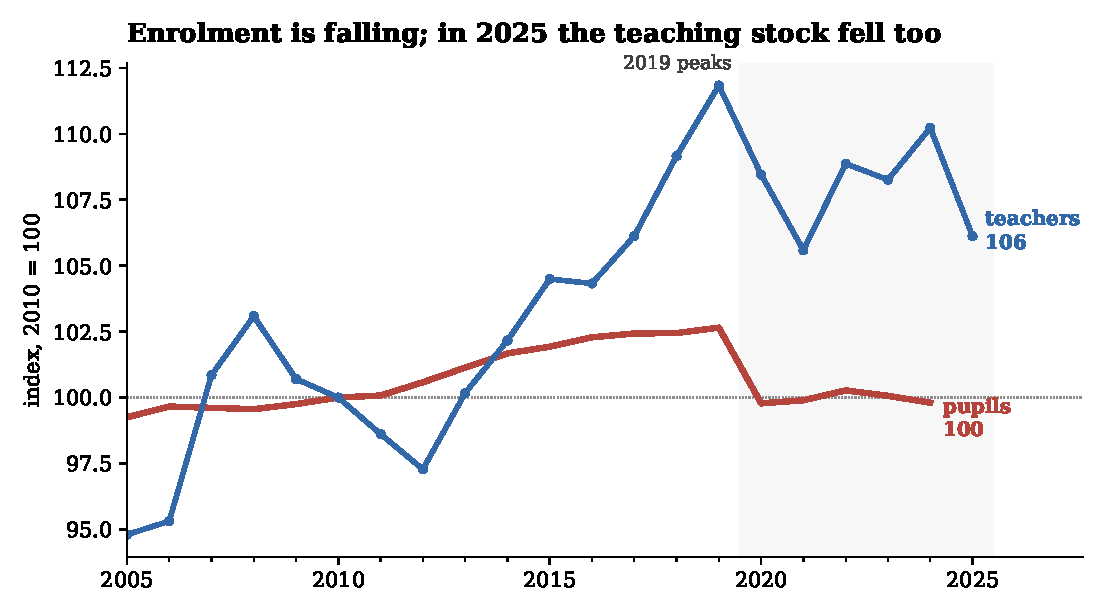
\includegraphics[width=0.9\textwidth]{figures/br_fig1_pupils_teachers.pdf}
  \caption{Public-school pupils and full-time qualified teachers, indexed
  to 2010.}
  \fignote{Teachers: CPS monthly data, employed K--12 teachers
  (occupations 2310--2330) with at least a bachelor's degree, annual
  average of weighted monthly stocks; survey estimates carry sampling
  error of roughly $\pm$1--2 per cent. The 2025 average covers eleven
  months --- no CPS was collected in October 2025 during the federal
  shutdown --- but the like-for-like eleven-month 2024 figure (4.52M)
  confirms the decline. Pupils: NCES, Digest of Education Statistics,
  table 203.10, fall enrolment in public schools.}
\end{figure}

In 2025 the workforce stopped ignoring it. The stock of qualified
teachers fell from 4.54 to 4.37 million --- 3.7 per cent, the sharpest
one-year drop in the series outside the pandemic itself. Some of this is
schools finally adjusting to smaller cohorts and the end of federal
relief money; districts that staffed up on ESSER funds are letting
attrition do the shrinking. But the composition of the change matters,
because the outflow is not being matched by a young inflow --- a point
Section~3 returns to.

\section*{2. Attrition is back to normal --- with an asterisk}

The headline number of the 2025 data is a good one. Of the teachers in
public-school classrooms in 2024, 7.9 per cent had left education
entirely a year later: not teaching, not working in a school, college or
any education-adjacent job. That is statistically indistinguishable from
the 2005--18 average of 7.7 per cent, and far below the 10.4 per cent
reached when the pandemic and the reopening chaos emptied classrooms
(Figure~2). By age, the picture is uniformly calmer: attrition among
teachers under 35, which spiked hardest after 2020, is back near its own
long-run norm, as is the mid-career trough and the retirement-driven rate
of the over-50s (Figure~3).

\begin{figure}[t]\centering
  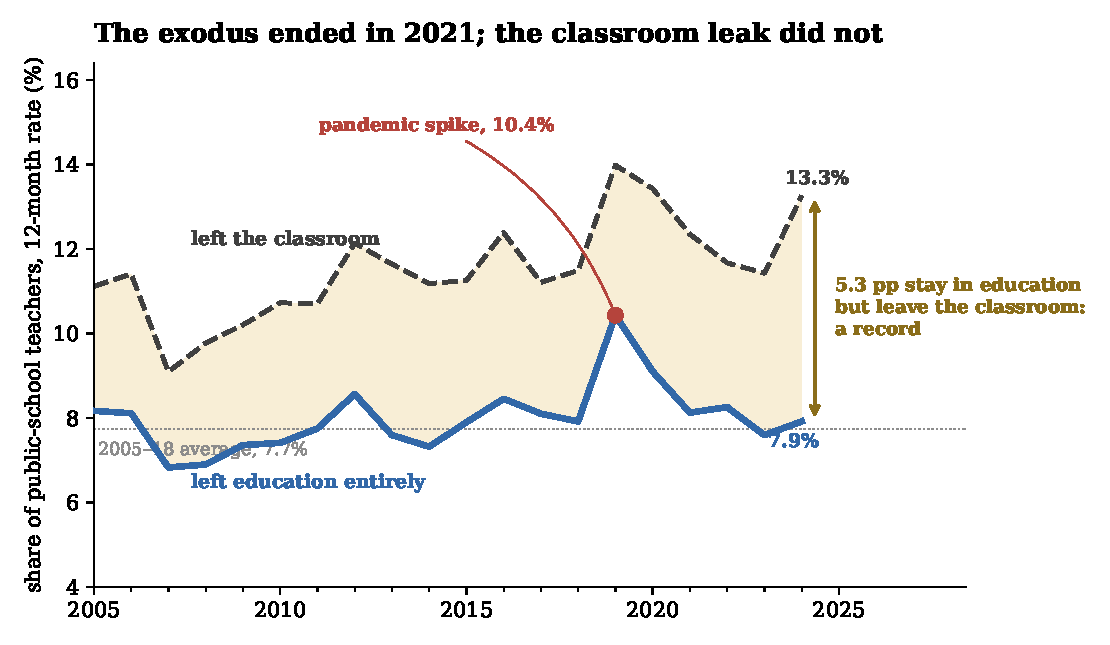
\includegraphics[width=0.9\textwidth]{figures/br_fig2_attrition.pdf}
  \caption{Two ways to leave: out of the classroom, and out of education.}
  \fignote{Public-school full-time K--12 teachers (BA+) followed twelve
  months in linked CPS interviews, 2005--2024 base years ($n=91{,}035$;
  2{,}841 in 2024, which lacks October links because no October 2025
  survey exists). Blue: no longer working in any education occupation at
  $t{+}12$ nor teaching at any later interview. Dashed: no longer a
  classroom teacher by the same standard. The gap between the lines is
  movement into other education work --- support roles, administration,
  post-secondary and other instruction.}
\end{figure}

\begin{figure}[t]\centering
  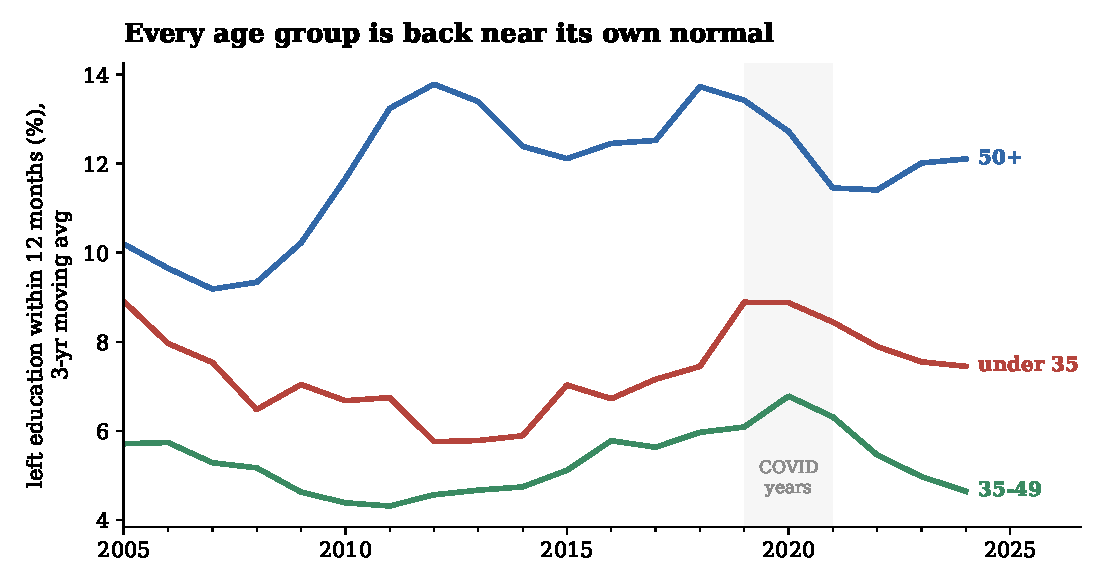
\includegraphics[width=0.9\textwidth]{figures/br_fig3_age.pdf}
  \caption{Attrition from education by age of teacher.}
  \fignote{Same universe and definition as the blue line of Figure 2,
  split by age at the base interview; three-year centred moving averages.
  The 50+ line embeds retirements and is structurally the highest.}
\end{figure}

The asterisk is the dashed line above it. Counting exits from the
\emph{classroom} rather than from education, attrition in 2024--25 was
13.3 per cent --- still roughly two points above its pre-pandemic norm,
and rising while the blue line fell. The wedge between the two lines,
teachers who stay in education but stop teaching, reached 5.3 percentage
points, the widest in twenty years of data; before the pandemic it
averaged 3.4. Two in five of last year's classroom leavers, in other
words, did not leave the sector: they became instructional coaches,
administrators, counselors, tutors, college instructors. For school
budgets this is churn; for pupils it is the same empty desk at the front
of the room. The post-pandemic exodus from education is over, but an
internal migration out of the classroom has replaced it --- and it does
not show up in the headline rate.

\section*{3. The inflow is running on career-changers}

Attrition is only half of the ledger. The other half --- who replaces the
leavers --- is where the 2025 data look least like a recovery. The median
teacher who entered a classroom between 2024 and 2025 was \emph{42 years
old}. Three quarters came directly from another job, a further 18 per
cent from outside the labour force, and fewer than one in five was under
30. Teaching in America is increasingly staffed at the margin by
mid-career adults --- returners circling back and professionals switching
in --- rather than by a pipeline of the young: the under-35 share of the
teaching stock has drifted down from about 32 per cent in the
mid-2000s to 29 per cent today, and one leaver in six is back in a
classroom within months, a revolving door that papers over the thinness
of genuinely new supply.

Career-changers are not worse teachers, and a workforce that can draw on
them is more resilient than one that cannot. But an inflow with a median
age of 42 buys fewer future teaching years per hire, arrives needing
certification flexibility the current systems ration, and --- crucially
--- responds to relative pay, which is the one margin that has moved in
the wrong direction for fifteen years.

\section*{4. Pay never came back}

Adjusted for inflation, the median full-time teacher earned \$1{,}380 a
week in 2025 against \$1{,}462 in 2010 --- 5.6 per cent less
(Figure~4). Over the same fifteen years the median wage of all workers
rose 9 per cent in real terms, and that of degree-holders rose 3 per
cent. Relative to the graduate labour market in which teachers are
actually recruited, teacher pay has slid from 87 to 79 cents on the
dollar. The inflation surge did the sharpest damage: between 2021 and
2023 teachers lost nearly 6 per cent of their real weekly pay, and the
partial rebound since has recovered less than half of it.

\begin{figure}[t]\centering
  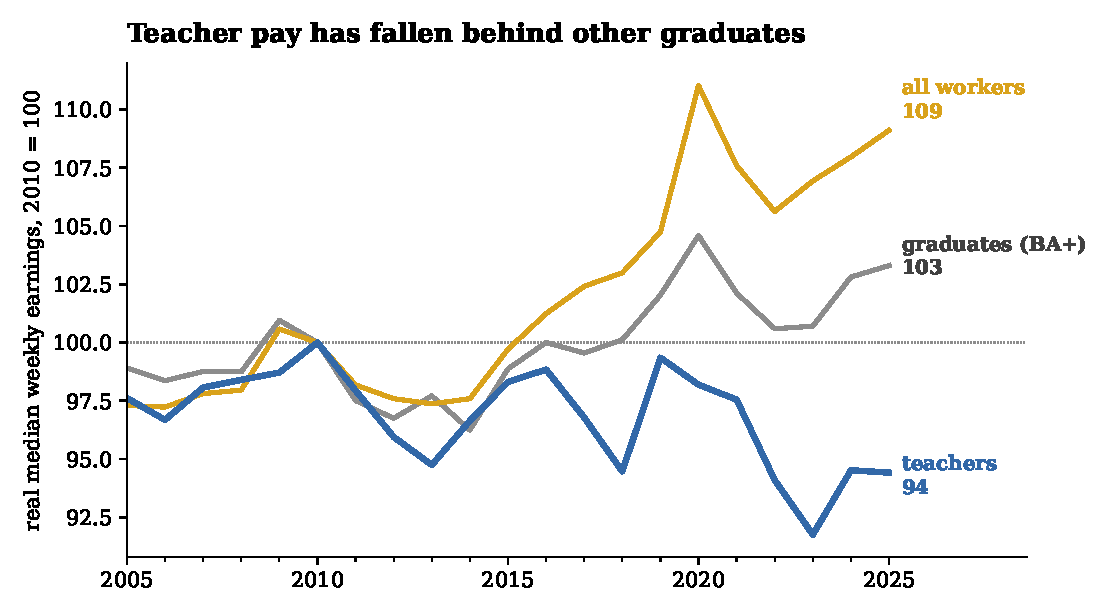
\includegraphics[width=0.9\textwidth]{figures/br_fig4_pay.pdf}
  \caption{Real median weekly earnings: teachers, all graduates, all
  workers.}
  \fignote{Teachers: weighted median usual weekly earnings of full-time
  K--12 teachers (BA+), CPS outgoing-rotation interviews, deflated by
  CPI-U. Graduates: BLS median usual weekly earnings, bachelor's degree
  and higher, age 25+. All workers: BLS real median usual weekly
  earnings, age 16+. Indexed to 2010 = 100.}
\end{figure}

A pay position like this coexists with normal attrition for one reason
only: the alternatives on offer. Which brings the story to its least
comfortable chart.

\section*{5. A recovery on loan}

Teacher retention in the United States moves with the temperature of the
labour market around it. Across two decades, the rate at which teachers
leave education tracks the private-sector quits rate --- the economy's
willingness to change jobs --- with a correlation of $+0.33$; teachers
stay put when everyone stays put (Figure~5). And the market has cooled
sharply: private quits have fallen from 3.1 per cent a month at the 2022
frenzy to 2.3 per cent, hiring rates are at post-2014 lows, and job
openings per unemployed worker are back below their pre-pandemic level.

At a 2.3 per cent quits rate, the historical relationship predicts
teacher attrition of almost exactly 8 per cent. Observed attrition:
7.9. The 2024 point sits precisely on the fitted line (Figure~5, right
panel). Today's normal attrition, in other words, is not evidence that
teaching has become more attractive --- pay says the opposite --- but
evidence that its competitors have become less so. It is retention
borrowed from a slack market, on terms set by the next expansion: the
same relationship implies that a return of quits to their 2022 level
would push attrition back up by half a point, before counting the
classroom-exit wedge and the grey inflow that a hot market would also
amplify.

\begin{figure}[t]\centering
  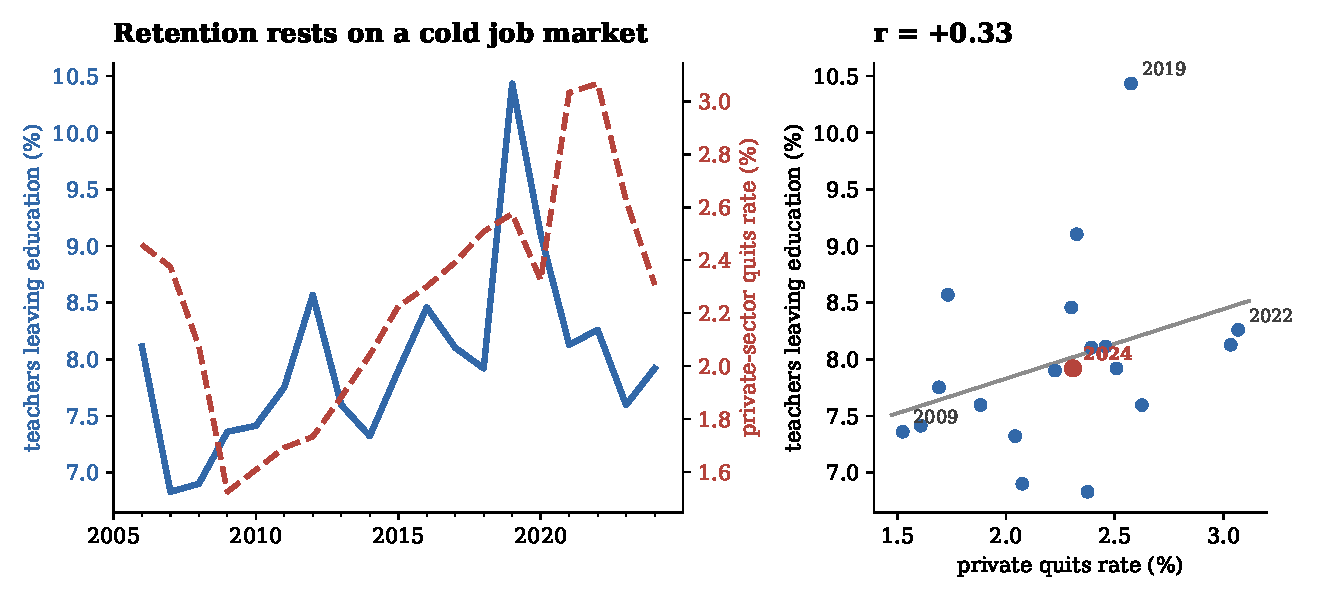
\includegraphics[width=\textwidth]{figures/br_fig6_market.pdf}
  \caption{Teacher attrition and the outside labour market.}
  \fignote{Left: teachers leaving education (as in Figure 2) and the
  private-sector quits rate (JOLTS, annual average of monthly rates).
  Right: the same two series as a scatter with an OLS fit; the 2024 point
  lies on the line. The 2019 observation links into 2020 and carries the
  COVID shock.}
\end{figure}

\section*{6. What this means}

Read quickly, the 2025 data close the book on the pandemic teacher
crisis: attrition normal, every age group settled, ratios improving. Read
carefully, they describe a workforce in remission, not in health. The
stock is now falling. The classroom is leaking into the back office at a
record rate. New supply is old, and thin among the young. Pay is eight
points further behind the graduate market than in 2010. And the
retention that looks so reassuring is fully explained by the coldest
hiring market in a decade.

None of those five facts is controlled by school systems' good luck
holding. One is: pay. The quiet years the labour market has lent are
precisely the window in which restoring teacher pay --- and making the
classroom itself a job people want to keep, not a stepping stone to the
jobs around it --- is cheapest, because retention does not need rescuing
at the same time. The data will say whether the window was used. On the
2025 vintage, it is still open, and still closing.

\vspace{8pt}
\begin{tcolorbox}[colback=white,colframe=ecgray,boxrule=0.6pt,
                  left=10pt,right=10pt,top=8pt,bottom=8pt]
{\footnotesize\textbf{Data and definitions.} Teacher series: CPS basic
monthly microdata, January 2005--December 2025 (Census Bureau; NBER
mirror before 2021). The CPS re-interviews each address twelve months
apart; persons are linked across interviews and validated on sex, race
and age progression (Madrian--Lefgren). Attrition (Figures 2, 3, 5):
public-school full-time K--12 teachers --- occupations 2310
(elementary/middle), 2320 (secondary), 2330 (special education) --- with
a bachelor's degree or higher, base rotations with re-interviews;
a leaver has left the classroom (dashed) or all education-adjacent
occupations (solid) at $t{+}12$ and is not observed teaching in any later
interview. This definition matches the NCES Teacher Follow-up Survey and
retrospective-CPS benchmarks (public-school leaver rates of 7.6--8.0 per
cent). Stocks and earnings use the full K--12 universe including private
schools. All estimates use final person weights. External series: NCES
Digest table 203.10 (enrolment); BLS via FRED --- LEU0252918500,
LEU0252881600 (comparator earnings), JTS1000QUR (quits), CPIAUCSL
(deflator). No CPS was collected in October 2025 (federal shutdown):
2025 stocks average eleven months and the 2024$\to$25 links exclude
October. Replication code: \texttt{src/30\_borrowed\_recovery\_data.py}
and \texttt{src/31\_borrowed\_recovery\_figures.py}.}
\end{tcolorbox}

\subsection*{References}
{\small
\hangindent=14pt Aldeman, C.\ and S.\ Yi (2025). Are Teachers Abandoning
Teaching? Data Show Teacher Turnover Remains Low. \emph{Education Next}.

\hangindent=14pt Durán Roa, J.\,E.\ (2026). \emph{Who Leaves Teaching, and
Why? The Profile of Teacher Attrition in the United States, 2005--2025}.
Mimeo, University of Alicante (companion paper, this repository).

\hangindent=14pt Education Policy Institute (2026). \emph{A borrowed
recovery: the 2025 school workforce data}. EPI, London.

\hangindent=14pt Harris, D.\,N.\ and S.\,J.\ Adams (2007). Understanding
the level and causes of teacher turnover: A comparison with other
professions. \emph{Economics of Education Review} 26(3), 325--337.

\hangindent=14pt Madrian, B.\ and L.\ Lefgren (2000). An approach to
longitudinally matching Current Population Survey respondents.
\emph{Journal of Economic and Social Measurement} 26(1), 31--62.

\hangindent=14pt National Center for Education Statistics (2024--25).
Teacher Follow-up Survey 2021--22; Digest of Education Statistics 2025.
U.S.\ Department of Education, Washington DC.
}

\end{document}
